\documentclass{beamer}
\usepackage[utf8]{inputenc}

\usetheme{Madrid}
\usecolortheme{default}
\usepackage{amsmath,amssymb,amsfonts,amsthm}
\usepackage{txfonts}
\usepackage{tkz-euclide}
\usepackage{listings}
\usepackage{adjustbox}
\usepackage{array}
\usepackage{tabularx}
\usepackage{gvv}
\usepackage{lmodern}
\usepackage{circuitikz}
\usepackage{tikz}
\usepackage{graphicx}

\setbeamertemplate{page number in head/foot}[totalframenumber]

\usepackage{tcolorbox}
\tcbuselibrary{minted,breakable,xparse,skins}



\definecolor{bg}{gray}{0.95}
\DeclareTCBListing{mintedbox}{O{}m!O{}}{%
  breakable=true,
  listing engine=minted,
  listing only,
  minted language=#2,
  minted style=default,
  minted options={%
    linenos,
    gobble=0,
    breaklines=true,
    breakafter=,,
    fontsize=\small,
    numbersep=8pt,
    #1},
  boxsep=0pt,
  left skip=0pt,
  right skip=0pt,
  left=25pt,
  right=0pt,
  top=3pt,
  bottom=3pt,
  arc=5pt,
  leftrule=0pt,
  rightrule=0pt,
  bottomrule=2pt,

  colback=bg,
  colframe=orange!70,
  enhanced,
  overlay={%
    \begin{tcbclipinterior}
    \fill[orange!20!white] (frame.south west) rectangle ([xshift=20pt]frame.north west);
    \end{tcbclipinterior}},
  #3,
}
\lstset{
    language=C,
    basicstyle=\ttfamily\small,
    keywordstyle=\color{blue},
    stringstyle=\color{orange},
    commentstyle=\color{green!60!black},
    numbers=left,
    numberstyle=\tiny\color{gray},
    breaklines=true,
    showstringspaces=false,
}
%------------------------------------------------------------
%This block of code defines the information to appear in the
%Title page
\title %optional
{5.8.10}
\date{October  2025}
%\subtitle{A short story}

\author % (optional)
{BEERAM MADHURI - EE25BTECH11012}



\begin{document}


\frame{\titlepage}
\begin{frame}{Question}
Narayan tells his daughter, `Seven years ago, I was seven times as old as you were then. Also, 3 years from now, I shall be 3 times as old as you will be.' Find their ages.
\end{frame}
 
\begin{frame}{given data}
 Let present age of Narayan $= N$ and \\
Present age of daughter $= D$. \\
7 years ago: 
\begin{align}
(N-7) = 7(D-7) \\
N-7 = 7D -49 \\
7D-N = 42
\end{align}
and 3 years from now: 
\begin{align}
(N+3) = 3(D+3) \\
N+3 = 3D +9\\
3D-N = -6 
\end{align}
\end{frame}

\begin{frame}{solution}
\frametitle{finding the present age of Narayan and his duaghter:}
expressing the given information in matrix form
\begin{align}
\begin{pmatrix}7 & -1 \\3 & -1\end{pmatrix}\begin{pmatrix}D \\N\end{pmatrix}=\begin{pmatrix}42 \\-6\end{pmatrix}
\end{align}
Augmented matrix:
\begin{align}
\left(\begin{array}{cc|c}7 & -1 & 42 \\3 & -1 & -6\end{array}\right)
\end{align}
\end{frame}
\begin{frame}
By row reductions:\\
\begin{align}
\begin{pmatrix}7 & -1 & | & 42 \\3 & -1 & | & -6\end{pmatrix}\xrightarrow{R_2 \rightarrow R_2 - \frac{3}{7} R_1}\begin{pmatrix}7 & -1 & | & 42 \\0 & -\frac{4}{7} & | & -24\end{pmatrix}\\
as \text{rank}(A) = \text{rank}(A|b) = 2
\end{align}
\begin{align}
\begin{aligned}N &= \frac{-24 \times 7}{-4} \\&= 42\end{aligned}\\
D = 12.
\end{align}
\end{frame}

\begin{frame}[fragile]
    \frametitle{Python Code}
    \begin{lstlisting}
import matplotlib.pyplot as plt
import numpy as np

# Create a range of x-values (Narayan's age) to plot over
# np.linspace creates an array of evenly spaced numbers over a specified interval
x = np.linspace(0, 60, 400)
# --- Define the Equations ---
# We rearrange the original equations to solve for y, the standard y = f(x) format for plotting.
\end{lstlisting}
\end{frame}

\begin{frame}[fragile]
\frametitle{python Code}
\begin{lstlisting}
# Equation 1 from "Seven years ago...": x - 7y = -42  =>  y = (x + 42) / 7
y1 = (x + 42) / 7

# Equation 2 from "Three years from now...": x - 3y = 6   =>  y = (x - 6) / 3
y2 = (x - 6) / 3
# --- Plotting the Graph ---

# Set up the plot size for better visibility
plt.figure(figsize=(10, 8))
\end{lstlisting}
\end{frame}

\begin{frame}[fragile]
\frametitle{python Code}
\begin{lstlisting}
# Plot the two lines representing the equations
plt.plot(x, y1, label='x - 7y = -42 (Seven years ago)')
plt.plot(x, y2, label='x - 3y = 6 (Three years from now)')

# --- Mark the Solution ---
# The solution to the problem is the single point where the two lines intersect.
# We can calculate this point algebraically and plot it.
intersection_x = 42
intersection_y = 12
plt.plot(intersection_x, intersection_y, 'ro', label=f'Intersection ({intersection_x}, {intersection_y})') # 'ro' means red circle
\end{lstlisting}
\end{frame}

\begin{frame}[fragile]
\frametitle{python Code}
\begin{lstlisting}
# --- Formatting the Graph for Clarity ---
# Add a title and labels for the x and y axes
plt.title("Graphical Solution to the Age Problem", fontsize=16)
plt.xlabel("Narayan's Current Age (x)", fontsize=12)
plt.ylabel("Daughter's Current Age (y)", fontsize=12)

# Display the legend to identify each line
plt.legend()
# Add a grid to make the coordinates easier to read
plt.grid(True, which='both', linestyle='--', linewidth=0.5)
\end{lstlisting}
\end{frame}

\begin{frame}[fragile]
\frametitle{python Code}
\begin{lstlisting}
# Set the visible range for the axes to focus on the solution area
plt.xlim(0, 50)
plt.ylim(0, 20)
# Add an annotation with an arrow to clearly point out the solution
plt.annotate(
    f'Solution: ({intersection_x}, {intersection_y})', # The text to display
    xy=(intersection_x, intersection_y),              # The point to annotate
    xytext=(intersection_x - 15, intersection_y + 3), # Where to place the text
    arrowprops=dict(facecolor='black', shrink=0.05),  # Arrow style
    fontsize=12
)
\end{lstlisting}
\end{frame}

\begin{frame}[fragile]
\frametitle{python Code}
\begin{lstlisting}
# Save the finished plot to a PNG image file
plt.savefig('age_problem_solution_graph.png')

print("Graph has been successfully generated and saved as age_problem_solution_graph.png")
\end{lstlisting}
\end{frame}

\begin{frame}[fragile]
\frametitle{C Code}
\begin{lstlisting}
 #include <stdio.h>
#include <math.h>

/*f(lambda) = (lambda + 6)^2 - (lambda + 2)^2 - 40
  We need f(lambda) = 0 */
double f(double lambda) {
    return (lambda + 6.0)*(lambda + 6.0)
         - (lambda + 2.0)*(lambda + 2.0)
         - 40.0;}
int main(void) {
    double left = -10.0;   // lower bound for search
    double right =  10.0;  // upper bound for search
    double mid;
    double tol = 1e-8;     // desired accuracy
\end{lstlisting}
\end{frame}

\begin{frame}[fragile]
\frametitle{C Code}
\begin{lstlisting}
#include <stdio.h>

int main() {
    int narayan_age, daughter_age;
    int solution_found = 0;

    // Let's iterate through possible ages.
    // We assume Narayan is older than his daughter.
    for (narayan_age = 1; narayan_age <= 150; narayan_age++) {
        for (daughter_age = 1; daughter_age < narayan_age; daughter_age++) {
\end{lstlisting}
\end{frame}

\begin{frame}[fragile]
\frametitle{C Code}
\begin{lstlisting}
 // Condition 1: Seven years ago, Narayan was 7 times his daughter's age.
 // (narayan_age - 7) == 7 * (daughter_age - 7)
 int is_condition1_met = (narayan_age - 7) == 7 * (daughter_age - 7);
// Condition 2: Three years from now, Narayan will be 3 times his daughter's age.
// (narayan_age + 3) == 3 * (daughter_age + 3)
int is_condition2_met = (narayan_age + 3) == 3 * (daughter_age + 3);
\end{lstlisting}
\end{frame}

\begin{frame}[fragile]
\frametitle{C Code}
\begin{lstlisting}
// If both conditions are true, we've found the answer.
if (is_condition1_met && is_condition2_met) {
printf("Solution Found:\n");
printf("Narayan's current age is: %d\n", narayan_age);
printf("Daughter's current age is: %d\n", daughter_age);
solution_found = 1;
break; // Exit the inner loop
            }
        }
\end{lstlisting}
\end{frame}

\begin{frame}[fragile]
\frametitle{C Code}
\begin{lstlisting}
    if (solution_found) {
            break; // Exit the outer loop
        }
    }
    if (!solution_found) {
        printf("No solution found within the specified age range.\n");
    }
    return 0;
}
\end{lstlisting}
\end{frame}

\begin{frame}[fragile]
\frametitle{Python and C Code}
\begin{lstlisting}
import ctypes

def main():
    narayan_age = ctypes.c_int()
    daughter_age = ctypes.c_int()
    solution_found = ctypes.c_int(0)
    for narayan in range(1, 151):
        for daughter in range(1, narayan):
            narayan_age.value = narayan
            daughter_age.value = daughter
\end{lstlisting}
\end{frame}

\begin{frame}[fragile]
\frametitle{Python and C Code}
\begin{lstlisting}
# Condition 1
is_condition1_met = (narayan_age.value - 7) == 7 * (daughter_age.value - 7)
 # Condition 2
is_condition2_met = (narayan_age.value + 3) == 3 * (daughter_age.value + 3)

if is_condition1_met and is_condition2_met:
print("Solution Found:")
print(f"Narayan's current age is: {narayan_age.value}")
print(f"Daughter's current age is: {daughter_age.value}")
solution_found.value = 1
break
\end{lstlisting}
\end{frame}

\begin{frame}[fragile]
\frametitle{Python and C Code}
\begin{lstlisting}
    if solution_found.value:
            break

    if not solution_found.value:
        print("No solution found within the specified age range.")

if __name__ == "__main__":
    main()

\end{lstlisting}
\end{frame}

\begin{figure}[H]
    \centering
    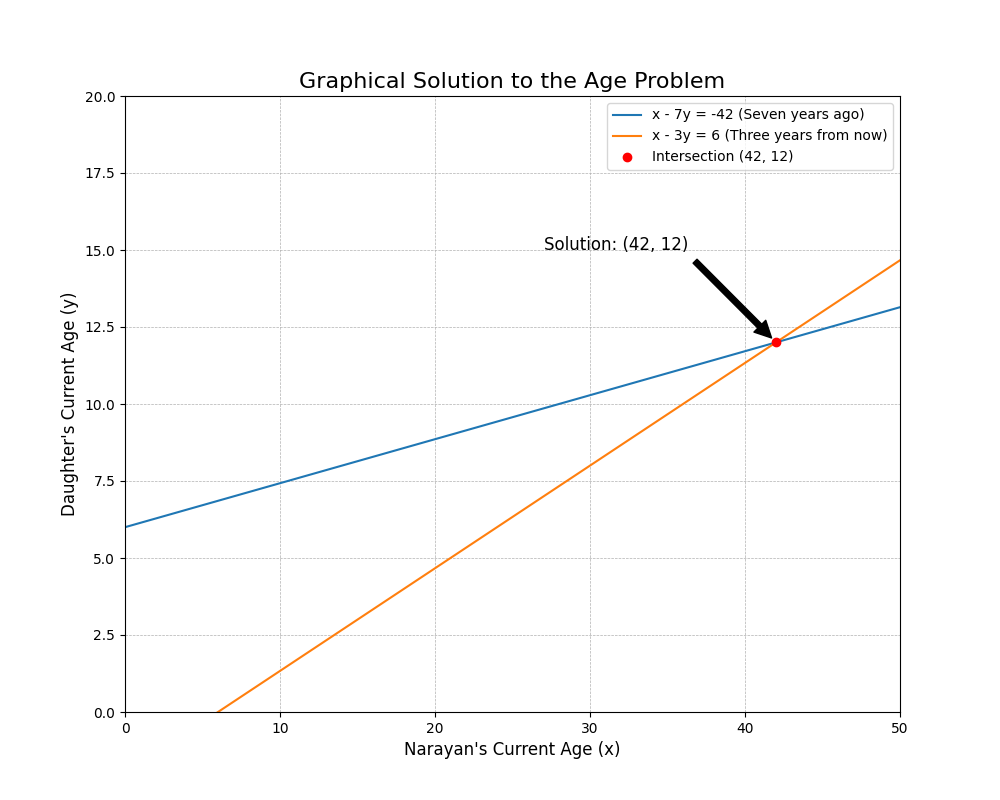
\includegraphics[width=0.7\columnwidth]{graph12.png}
    \caption{Plot}
    \label{fig:placeholder}
\end{figure}


\end{document}